% PNAS Nexus Research Report -- cross-country validity revision.
% Compile: pdflatex main; bibtex main; pdflatex main; pdflatex main.
\documentclass[unnumsec,webpdf,modern,large]{oup-authoring-template}
\usepackage{xurl}
\usepackage{booktabs}
\providecommand{\societylogo}{}
\graphicspath{{figures/}}
\journaltitle{PNAS Nexus}
\DOI{DOI added during production}
\copyrightyear{2026}
\pubyear{2026}
\access{Advance Access Publication Date: Day Month Year}
\appnotes{Research Report}

\title[Compressed preference geometry in synthetic publics]{Language models compress human preference geometry while political structure remains prompt-sensitive}
%Prompt-sensitive synthetic-public fidelity]{Language models compress policy-choice geometry while political structure remains prompt-sensitive in Chile, France, and Brazil

\author[1,2,$\ast$]{Adolfo Ignacio Fuentes-Jofre}
\author[1,2,3,$\ast$]{Cristian Candia}

\address[1]{\orgdiv{Computational Research in Social Science Laboratory},
\orgname{School of Engineering, Universidad del Desarrollo},
\orgaddress{Las Condes, \postcode{7610658}, \country{Chile}}}
\address[2]{\orgdiv{Instituto de Data Science, Facultad de Ingenier\'ia},
\orgname{Universidad del Desarrollo},
\orgaddress{Las Condes, \postcode{7610658}, \country{Chile}}}
\address[3]{\orgdiv{Northwestern Institute on Complex Systems (NICO)},
\orgname{Northwestern University},
\orgaddress{Evanston, \state{IL}, \postcode{60208}, \country{USA}}}
\corresp[$\ast$]{Corresponding authors: Adolfo Ignacio Fuentes Jofr\'e, adolfo.fuentes.j@gmail.com; Cristian Candia, crcandiav@gmail.com.}


\abstract{
Large language models are increasingly used to construct synthetic publics. Prior work has documented errors in individual responses, population heterogeneity, and prompt robustness, but whether these failures reflect a common loss of fidelity or distinct properties of synthetic populations remains unclear. We tested this using matched pairwise policy choices from 1,991 Chilean, 843 French, and 434 Brazilian adults replayed through three open-weight model families. Across a 27-condition Chilean grid and cross-country factorial replications, no condition jointly reproduced individual choices, population heterogeneity, and political organization. The most consistent result was compression of the latent preference space: synthetic participant variance was only 0.4--10.5\% of the corresponding human reference in the primary comparisons and remained below human variance in all 270 matched refits. Political structure was much more sensitive to how choices were elicited. Reversing proposal position changed 12.3--31.2\% of decoded choices. Explicitly labeling the endpoints of the numeric left-right self-placement scale changed 20.5--28.1\% of choices and moved an independent proposal-level measure of left-right cleavage toward the human pattern in all three settings. Yet matched agreement improved by only 3.1--4.2 percentage points and participant geometry remained compressed. In Chile, the same intervention compressed the synthetic population further. These results separate political legibility from population fidelity: language models can recover salient political divisions while failing to preserve the breadth of human preference variation. Synthetic-public fidelity is therefore a property of the checkpoint, prompt, and setting, not of a checkpoint alone, and must be evaluated separately at individual, population, and political-structure levels.
}

\keywords{large language models, synthetic populations, survey simulation, population heterogeneity, prompt sensitivity}
\keywords[Classification]{Social Sciences; Computer Sciences}
\keywords[Abbreviations]{LLM, large language model; CI, confidence interval; UUID, universally unique identifier; ROC AUC, receiver-operating-characteristic area under the curve; CV, cross-validation; BT, Bradley--Terry; DYNAMAP, Dynamic System for Mapping of Users and Their Preferences Using Artificial Intelligence}

\otherabstract[Significance statement]{
Synthetic publics generated by language models may reproduce recognizable political patterns without preserving the diversity of the human populations they are intended to represent. Across matched policy choices from adults in Chile, France, and Brazil, synthetic participants occupied much narrower preference spaces than humans, while individual choices and political structure remained sensitive to proposal position and prompt wording. Explicitly labeling the ends of a political self-placement scale made political divisions more human-like but did not restore population heterogeneity. These findings show that political legibility and population fidelity are distinct properties. Evaluations of synthetic publics should therefore distinguish individual-choice agreement, population heterogeneity, positional stability, and political organization rather than treating any single measure as evidence of human-like representation.}

\begin{document}
\maketitle

\section{Introduction}

Large language models are increasingly used to answer surveys, forecast choices, and instantiate synthetic populations. Their value is often framed as \emph{algorithmic fidelity}: conditional model behavior may reproduce patterns observed among corresponding human groups \citep{Argyle2023}. Early work also showed that LLM-based participants can replicate some established behavioral findings \citep{Aher2023}, while political applications have used them to predict pairwise preferences or augment aggregate estimates \citep{GudinoRosero2024}. These successes motivate synthetic-public applications, but they do not by themselves establish population fidelity. A synthetic public may reproduce an aggregate mean while failing to preserve the choices of matched individuals, the heterogeneity among people, or the political divisions that organize those differences.

Existing evidence gives reason to separate these targets. Plausible averages can coexist with too little variation and altered covariate relationships \citep{Bisbee2024}. Identity-conditioned outputs can flatten or misrepresent demographic groups, and increased sampling temperature does not necessarily restore the missing variation \citep{Wang2025}. Other studies similarly report under-dispersion in voting preferences and contraction of persona-conditioned behavioral spaces \citep{Ball2025,Xiao2026,Bhattacharyya2026}. Even methods specialized to reproduce survey-response distributions improve some aggregate targets while continuing to struggle on unseen questions and countries \citep{Cao2025}. Population heterogeneity therefore requires direct validation rather than inference from average agreement or predictive accuracy.

A second challenge is specification dependence. Survey-style LLM responses can change under wording perturbations that do not produce corresponding changes in humans \citep{Tjuatja2024}, and closed-ended survey simulations differ materially across response-generation methods at both individual and subpopulation levels \citep{Ahnert2026}. For synthetic publics, this implies that substantive conclusions should not be inferred from one prompt realization alone. Position stability and prompt specification must be evaluated separately from human agreement: exchanging A/B placement should not alter the underlying proposal preference, while clarifying the meaning of a supplied political scale may reveal whether an apparent political structure depends on how that scale is expressed.

A third challenge is transfer across societies. Some evidence is encouraging: synthetic participants can approximate aggregate human responses in both WEIRD and non-WEIRD samples, although correspondence can be weaker outside the United States \citep{Shrestha2024}. Other work documents unevenly represented opinions, cultural tendencies, and cross-societal differences in LLM-simulated public opinion \citep{Santurkar2023,Atari2023,Brinkmann2023,Lu2025,Abeliuk2026}. Together with the difficulty of generalizing survey-response distributions to unseen countries \citep{Cao2025}, this means that fidelity established in one political and linguistic setting cannot simply be assumed to transfer to another.

Taken together, this literature implies a stricter validation problem than a single accuracy benchmark. A synthetic public should be evaluated on three separable requirements: whether it preserves matched behavior and population heterogeneity, whether its substantive structure is stable to prompt and position specification, and whether the same diagnostic pattern recurs across settings. We operationalize these requirements with seven criteria. \emph{Internal reconstruction} asks whether a spatial model explains an LLM's own repeated choices. \emph{Matched human agreement} asks whether the LLM selects the proposal chosen by the corresponding person. \emph{Self-placement recoverability} asks whether choice-derived coordinates encode supplied political self-placement. \emph{Position stability} asks whether changing A/B placement changes the decoded proposal choice. \emph{Participant geometry} asks whether synthetic people span the human latent space; \emph{proposal topology} asks whether relations among policy items are preserved; and \emph{political cleavage} asks whether the same proposals divide left- and right-identified groups. We estimate participant and proposal geometry using DYNAMAP (Dynamic System for Mapping of Users and Their Preferences Using Artificial Intelligence), a two-dimensional neural comparative-choice model that jointly embeds participants and policy proposals from repeated pairwise choices. Its architecture, estimation, alignment, and validation are specified below and in the SI Appendix (\textit{DYNAMAP architecture and validation}). Aggregate proposal structure and political cleavage are additionally evaluated with embedding-independent Bradley--Terry models.

The empirical design applies these criteria to the same matched decisions among confirmed adults. A Chilean grid replayed 39,820 choices---20 from each of 1,991 participants---with nine instruction-tuned checkpoints from Qwen3, Gemma 4, and Ministral 3 at three temperatures. Open-weight checkpoints were used so exact revisions and local inference settings could be fixed and replayed. We then selected three temperature-zero checkpoints that represented different grid maxima and crossed self-placement present versus ablated with original versus content-and-position-inverted A/B display. Checkpoint selection was outcome-informed; the $2\times2$ intervention was fixed before its new responses were generated. The same factorial was replicated in French and Brazilian Portuguese among 843 and 434 confirmed-adult participants, respectively, because a common data architecture captured pairwise policy choices around the 2022 presidential elections in two additional national and linguistic settings \citep{Navarrete2024}. The design therefore replays native-language policy instruments across three linguistic and national political settings; it provides cross-national replication, not representative coverage of languages or countries. Finally, after observing the bare-numeric results, we directly tested one candidate mechanism by explicitly labeling the endpoints of the self-placement scale for Qwen3-32B at temperature zero in both proposal orders. This outcome-informed probe tests whether clarifying the meaning of the supplied political scale alters political organization, without assuming that any such effect generalizes across checkpoints.

\section{Results}

\subsection{No model condition optimized all fidelity criteria}

All 27 grid conditions used the same 1,991 confirmed-adult participants, 20 decisions per participant, prompt template, and downstream estimators. Comparisons within the grid are therefore matched on people and proposals, although cross-family differences remain descriptive because checkpoint training, serving software, and numerical representation were not experimentally standardized.

Matched human agreement ranged from 0.510 to 0.571 (Fig.~\ref{fig:grid}; SI Appendix, Table~S2). Gemma 4-12B at $T=0$ had the highest agreement (0.571), but even this condition disagreed with the observed person in approximately 43\% of cells. Family averages were 0.558 for Gemma 4, 0.536 for Qwen3, and 0.530 for Ministral 3.

Internal reconstruction favored a different condition. Qwen3-14B at $T=0.7$ reached the highest raw DYNAMAP validation accuracy (0.850), but the condition-specific majority rule already achieved 0.809, leaving only about 0.040 lift. Gemma 4-31B at $T=0.7$ instead produced the largest lift (0.268) with lower raw accuracy. High reconstruction could therefore arise from concentrated responses rather than richer participant--proposal structure.

Recoverability of political self-placement produced another ordering. The human-coordinate benchmark classified held-out left (1--4) versus right (6--10) self-placement with 0.674 accuracy, compared with 0.516 from sociodemographics alone. The fixed adult holdout contained 199 majority-class participants among 347 (0.573). Qwen3-32B at $T=0$ reached 0.925 held-out and 0.912 CV-10 accuracy. These above-human scores reflect consistent use of an explicitly supplied persona cue, not emergent inference or deeper knowledge of individuals. Qwen3-32B at $T=0$, for example, recovered 59.4\% of the human left--right centroid separation but agreed with humans in only 52.3\% of cells. Gemma 4-12B at $T=0$ reached 57.1\% agreement but 39.4\% of human separation. Neither model scale nor temperature improved all criteria monotonically. No condition jointly maximized internal learnability, matched behavior, political organization, and human-like structure.

\begin{figure*}[t]
\centering
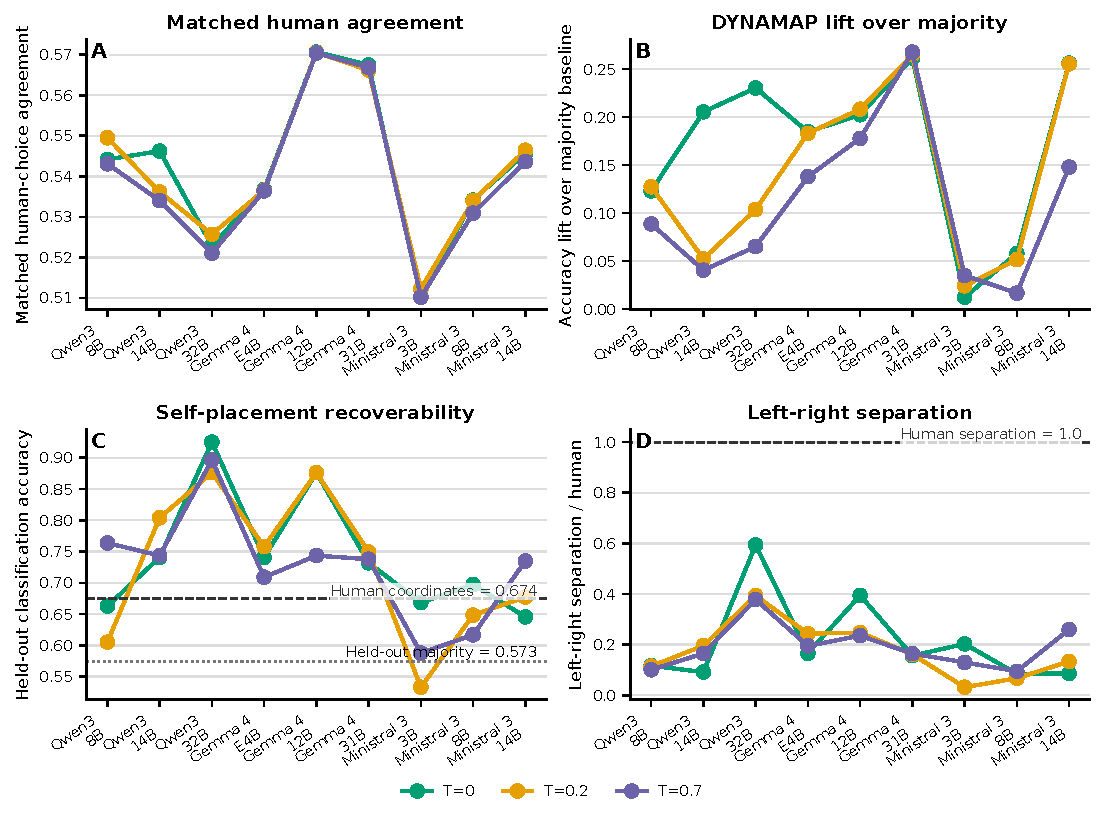
\includegraphics[width=0.98\textwidth]{figure1_model_grid_core_metrics.pdf}
\caption{Family, scale, and temperature move fidelity criteria differently. Each point summarizes one matched 39,820-decision confirmed-adult condition. Panel A compares model and human choices. Panel B subtracts the condition-specific validation-majority accuracy from internal DYNAMAP reconstruction. Panel C predicts supplied left--right self-placement from sociodemographics plus choice-derived coordinates; the dotted reference is the 0.573 majority rule in the fixed adult holdout. Panel D normalizes left--right separation to the independently fitted adult human space after proposal-anchor alignment. Geometry panels use the primary DYNAMAP initialization (seed 101). Dashed benchmarks are labeled as human references. Lines connect checkpoint sizes only to aid reading; they do not imply a continuous scale law.}
\label{fig:grid}
\figalttext[Four panels of metrics across 27 model conditions]{Lines for three temperatures vary nonmonotonically across nine family-size cells. The maxima for human agreement, DYNAMAP lift, political self-placement classification, and left-right separation occur in different conditions.}
\end{figure*}

\subsection{Synthetic participants occupied a small fraction of the human space}

We aligned each independently fitted synthetic space to the human space using only matched proposal coordinates; political self-placement did not enter the transformation. At the primary initialization (seed 101), synthetic participant-coordinate variance was 0.4--6.2\% of the human value across the Chilean grid, while correlations between human and synthetic proposal distances were only 0.023--0.136. Contraction appeared in every family. Because proposal-anchor alignment removes arbitrary orientation and scale before comparing participant coordinates, it cannot be attributed merely to rotation of a latent space.

Fig.~\ref{fig:geometry_compression} illustrates the human space and the three temperature-zero checkpoints subsequently used in the factorial. The examples were chosen because they represented different grid maxima in the original condition-selection exercise: Gemma 4-12B for matched agreement, Qwen3-32B for self-placement recoverability, and Ministral 3-14B for reconstruction lift. All three synthetic participant clouds occupy a small region of the aligned adult human space. Qwen3-32B exhibits a more visible supplied left--right axis than the other examples, yet its total participant variance remains 6.2\% of human. Recovering one direction did not restore the breadth or topology of the human population. The compression result also survives the 30-seed analysis reported below.

\begin{figure*}[t]
\centering
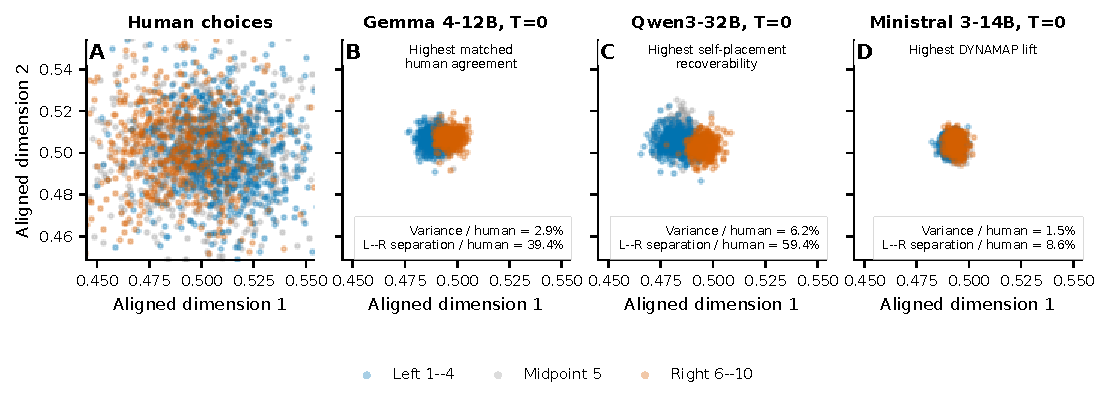
\includegraphics[width=0.98\textwidth]{figure3_aligned_coordinate_distributions.pdf}
\caption{Synthetic participant coordinates occupy a small fraction of the human latent space. Panel A shows matched human participant coordinates. Panels B--D show Gemma 4-12B at $T=0$ (highest matched human agreement), Qwen3-32B at $T=0$ (highest self-placement recoverability), and Ministral 3-14B at $T=0$ (highest DYNAMAP lift). Synthetic proposal coordinates were aligned to matched human proposal anchors with a similarity Procrustes transformation, and the fitted transformation was applied unchanged to participant coordinates. Political self-placement was not used for alignment. All panels share axes; annotations report total participant-coordinate variance and left--right centroid separation as percentages of the human reference. Estimates use the primary DYNAMAP initialization (seed 101).}
\label{fig:geometry_compression}
\figalttext[Four aligned latent-space maps with shared axes]{Human participants occupy a broad two-dimensional cloud. The three selected synthetic populations occupy much smaller regions, although Qwen3-32B shows the clearest supplied left-right separation.}
\end{figure*}

\subsection{Position and self-placement interventions exposed distinct fragilities}

The factorial crossed the three temperature-zero checkpoints with self-placement present versus ablated and original versus inverted A/B order. Each of the 12 cells contained the same 1,991 confirmed-adult participants and 39,820 decisions. DYNAMAP accuracy remained 0.763--0.827 and lift over the validation-majority rule 0.130--0.267, so every intervention cell remained internally learnable.

Internal learnability did not imply position invariance (Fig.~\ref{fig:confirmatory}A; SI Appendix, Tables~S3--S5). After decoding both displays to original proposal identity, cross-order agreement was 0.688--0.834: reversing content and position changed 16.6--31.2\% of substantive choices. Participant-bootstrap intervals were narrow; intervals that additionally varied proposal composition were wider but preserved the diagnosis (SI Appendix, Fig.~S18).

The self-placement intervention revealed a different dependence (Fig.~\ref{fig:confirmatory}B--C). Including self-placement increased held-out political self-placement classification accuracy by 0.124--0.386 in all six model-by-order contrasts, yet reduced matched human agreement in all six comparisons. With the cue ablated, held-out classification fell to 0.522--0.559 in all six cells, below the 0.573 majority rule; the recovered axis was therefore the supplied one. For Qwen3-32B in original order, held-out self-placement accuracy reached 0.925 while matched agreement was 0.523 and participant-coordinate variance was 6.2\% of human. Self-placement recoverability, matched-choice fidelity, and population heterogeneity therefore moved separately.

\begin{figure*}[t]
\centering
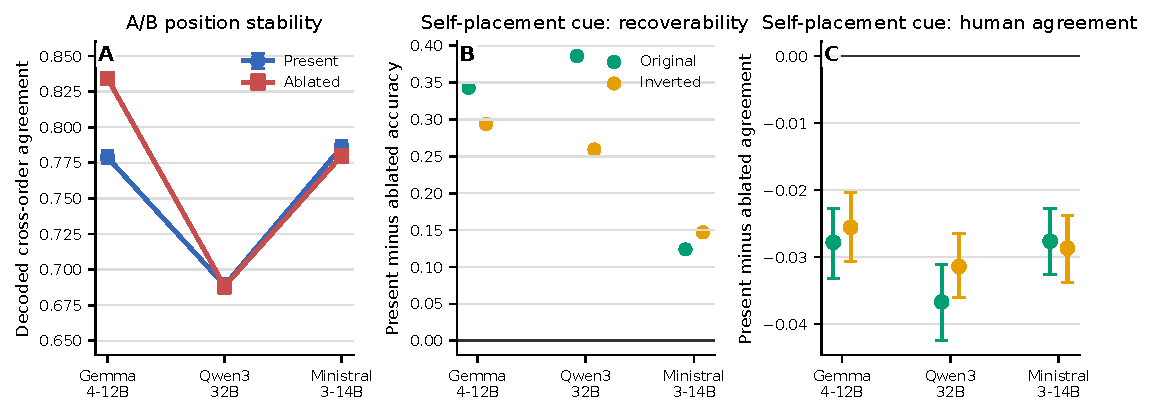
\includegraphics[width=0.98\textwidth]{figure_confirmatory_validity.pdf}
\caption{Factorial interventions separate position stability, self-placement recoverability, and matched human agreement in the confirmed-adult cohort. Panel A shows agreement between original and inverted A/B displays after responses were decoded to original proposal identity; intervals resample paired participant histories. Panels B--C show the effect of including self-placement (present minus ablated) on held-out political self-placement classification and matched human agreement within each A/B order. Panel B reports deterministic fixed-holdout point contrasts; panel C intervals use paired participant-bootstrap resampling.}
\label{fig:confirmatory}
\figalttext[Three panels summarizing two factorial interventions]{Cross-order agreement ranges from about 0.69 to 0.83. Including self-placement increases held-out political self-placement classification accuracy for every model and order but decreases matched human agreement in every comparison.}
\end{figure*}

\subsection{Compression recurred in France and Brazil}

We replicated the factorial in the primary 20-choice cohorts in France and Brazil (Fig.~\ref{fig:country_replication}). Across the 24 country-by-checkpoint-by-prompt-by-order cells, DYNAMAP reconstruction remained within the range observed in Chile, while lift extended above it (0.200--0.331 against a Chilean maximum of 0.268; SI Appendix, Table~S10). Internal learnability therefore persisted outside Chile but again did not establish matched human fidelity.

Because released French and Brazilian rows place the selected proposal first, original-order agreement is outcome-informed. We therefore averaged equally across the four decoded prompt-by-order cells (Fig.~\ref{fig:country_replication}A). Treatment-balanced agreement was 0.651--0.687 in France and 0.572--0.636 in Brazil. These levels should not be ranked across countries because the instruments contain different proposal catalogues and the released-file order is not a common randomized display. Cross-order proposal-identity consistency ranged from 0.698 to 0.877 (Fig.~\ref{fig:country_replication}B), so inversion changed 12.3--30.2\% of substantive choices. The order-averaged displayed-A rate---the relevant positional statistic under selected-first release order---ranged from 0.36 to 0.64 (SI Appendix, Table~S10): Gemma and Qwen concentrated on visible A, whereas Ministral concentrated on B. Equal weighting across orders is therefore essential.

At the primary DYNAMAP initialization (seed 101), participant-level compression also persisted (Fig.~\ref{fig:country_replication}C--D). After equal weighting across the four factorial cells, artificial variance was 8.6--10.5\% of the French adult human reference and 2.5--4.3\% of the Brazilian reference. The directional left--right separation diagnostic retained 18.2--36.3\% of the French reference and 4.0--11.1\% of the Brazilian reference at this initialization, but it varied across DYNAMAP seeds and between the C10 and C20 cohorts and is not used to rank checkpoints. Compression therefore recurred outside Chile, but its magnitude and accompanying topology did not. The final Results section tests whether these political differences survive explicit verbal scale endpoints.

\begin{figure*}[t]
\centering
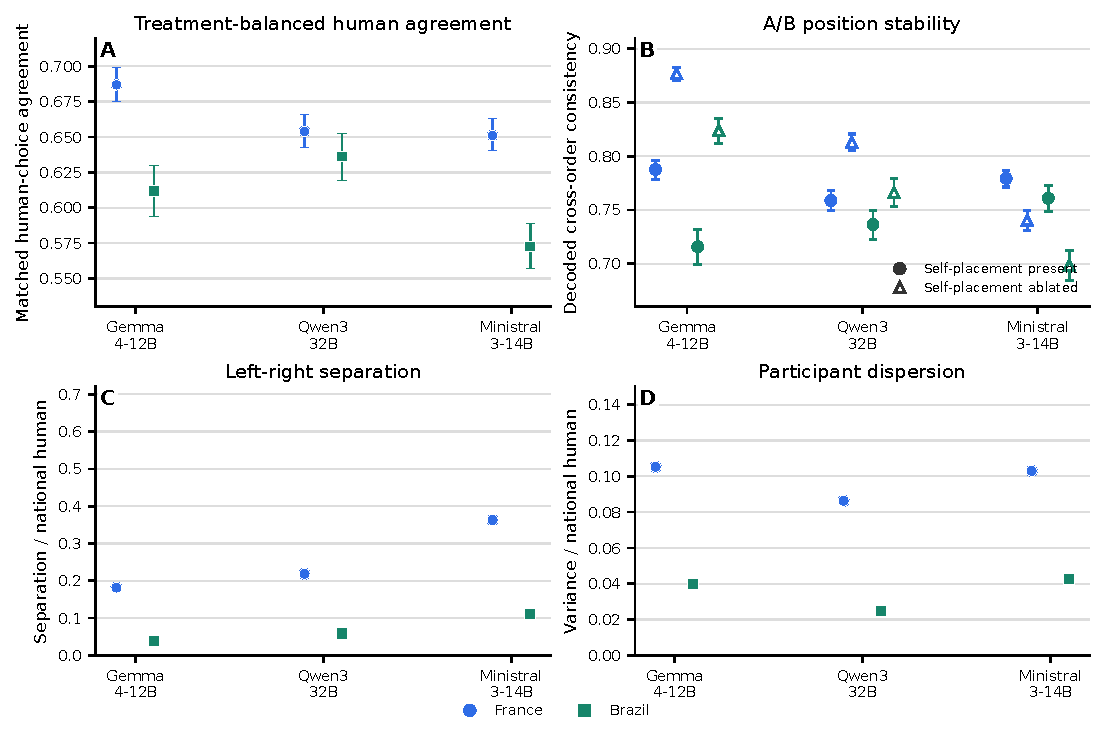
\includegraphics[width=0.98\textwidth]{figure4_cross_country_behavior_geometry.pdf}
\caption{Behavioral and geometric replication in the primary confirmed-adult French and Brazilian C20 cohorts. Panel A shows equal-weight decoded matched human agreement with participant-bootstrap 95\% confidence intervals; absolute levels are not compared across countries because instruments and released-file order differ. Panel B shows proposal-identity consistency across original and inverted displays with self-placement present (filled circles) or ablated (open triangles). At the primary DYNAMAP initialization (seed 101), panels C--D normalize left--right centroid separation and total participant-coordinate variance to each country's own adult human space after proposal-anchor alignment. The separation diagnostic is not a checkpoint ranking. French and Brazilian spaces were aligned only to their national reference and never to one another. Reconstruction and lift appear in SI Appendix, Table~S10.}
\label{fig:country_replication}
\figalttext[Four panels comparing behavior and normalized geometry in France and Brazil]{Treatment-balanced matched agreement and A/B identity consistency vary by checkpoint and setting. At seed 101, synthetic left-right separation and especially participant variance remain below the corresponding national human references.}
\end{figure*}

\subsection{Human benchmarks and initialization robustness bounded the claim}

The same 3,982 held-out Chilean decisions 19--20 placed LLM agreement beside a common set of adult human reference predictors (Fig.~\ref{fig:validity}A--B). Balanced random choice was 0.500 by construction and a training-set marginal A/B rule reached 0.509; Bradley--Terry proposal popularity reached 0.679, a sociodemographic-plus-proposal predictor reached 0.687, and human DYNAMAP reached 0.662. The factorial LLM conditions reached 0.530--0.614. Human DYNAMAP is a structural reference for out-of-sample predictability, not a normative ceiling.

Across 30 independent DYNAMAP initializations, participant-coordinate variance remained below the same-seed human reference in all 270 synthetic fits (Fig.~\ref{fig:validity}C; SI Appendix, Table~S16 and Fig.~S15). This robustness concerns neural-network optimization initialization; it does not quantify LLM-generation, participant-sampling, or proposal-sampling uncertainty.

\begin{figure*}[t]
\centering
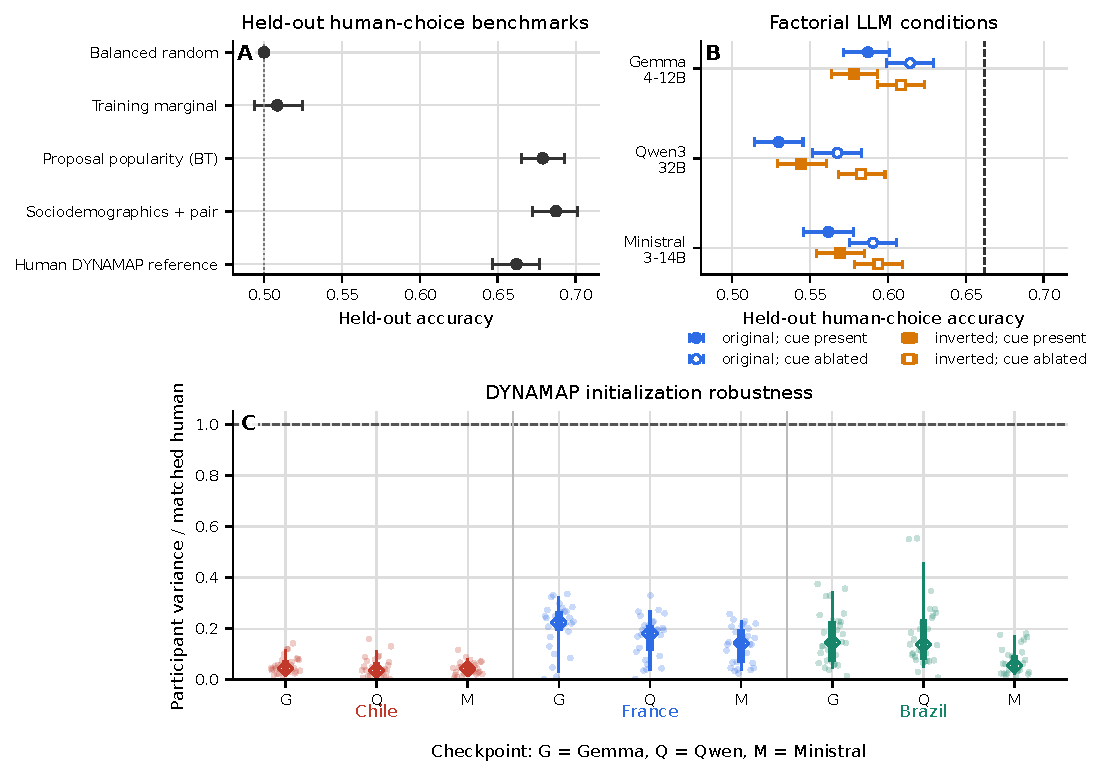
\includegraphics[width=0.98\textwidth]{figure5_human_benchmarks_multiseed.pdf}
\caption{Human benchmarks and initialization robustness bound the claim. Panel A compares five human-choice reference predictors trained on decisions 1--18 and evaluated on decisions 19--20; balanced random choice is an analytic 0.500 reference without sampling uncertainty. Panel B places all 12 factorial LLM conditions on the same held-out agreement scale; the human DYNAMAP line is a structural reference rather than a human ceiling. Panel C shows participant-coordinate variance relative to the matched same-seed human fit across 30 DYNAMAP initialization seeds for nine country-by-checkpoint groups; thin ranges span the 5th--95th percentiles, thick ranges the interquartile range, diamonds the median, and faint points individual seeds.}
\label{fig:validity}
\figalttext[Three panels of benchmarks and initialization sensitivity]{LLM held-out agreement is below three fitted human predictors. Across 30 DYNAMAP seeds, every synthetic participant-variance estimate is below the matched human reference.}
\end{figure*}

\subsection{Verbal endpoint anchors changed political direction without restoring population geometry}

The bare-numeric prompts produced different political-cleavage patterns across settings, but those patterns were not stable attributes of a checkpoint. We tested a documented prompt-specification mechanism with Qwen3-32B at $T=0$, the focal condition that made supplied self-placement most recoverable in Chile. For the same adult C20 participants, proposals, model revision, decoding parameters, and original or inverted display, the only intervention was to append verbal scale endpoints: extreme left and extreme right in each prompt's native language. Because this mechanism probe was designed after observing the bare-prompt pattern and uses one checkpoint, it diagnoses sensitivity rather than providing a second model comparison (Fig.~\ref{fig:endpoint_anchor}; SI Appendix, Table~S19 and Figs.~S19--S21).

The wording change was behaviorally consequential. Averaged equally across proposal orders, anchors changed 28.1\% [27.4\%, 28.8\%] of Chilean, 20.5\% [19.7\%, 21.2\%] of French, and 22.4\% [21.3\%, 23.6\%] of Brazilian choices. Matched human agreement increased by only 4.2, 3.1, and 3.7 percentage points, respectively, but the order-specific effects were $+5.0/+3.4$ in Chile, $+12.1/-6.0$ in France, and $+13.2/-5.8$ in Brazil (original/inverted, percentage points). Thus, the French and Brazilian average gains were concentrated in the outcome-informed released original order and reversed after inversion. Anchored cross-order change was 25.5\% in Chile, 37.5\% in France, and 43.1\% in Brazil; the latter two exceeded the 12.3--30.2\% factorial range. A more explicit political scale therefore did not make choices position-invariant.

The independent Bradley--Terry comparison nevertheless showed that the supplied axis was interpreted differently. In Chile, human--model cleavage correlation changed from $-0.442$ to 0.409 in original order and from $-0.474$ to 0.388 after inversion. France moved from 0.494 to 0.828 and from 0.228 to 0.601; Brazil moved from 0.410 to 0.772 and from 0.039 to 0.599. Verbal endpoints thus moved proposal-level political division toward the human direction in every setting and order. Magnitude did not return to equality: anchored synthetic-to-human RMS ratios were 2.66/2.67 in Chile, 1.56/1.20 in France, and 1.43/1.07 in Brazil (original/inverted). Cleavage remains informative as an embedding-independent diagnostic, but its level and direction cannot be treated as a fixed country or checkpoint signature.

DYNAMAP sharpened the distinction between political legibility and population geometry. At the primary initialization (seed 101), anchors increased held-out self-placement accuracy from 0.925 to 0.968 in original-order Chile, 0.792 to 0.824 in France, and 0.761 to 0.915 in Brazil; the inverted-order gains were also positive. In Chile, greater legibility coincided with further compression: participant-coordinate variance fell from 6.2\% and 1.9\% under bare prompts to 1.6\% and 0.4\% with anchors in original and inverted orders. Across anchored orders, variance remained 8.7--28.1\% of the French and 3.2--18.5\% of the Brazilian human reference. The original-order expansions in France and Brazil did not generalize to the inverted display, and one-dimensional separation effects varied across initialization seeds. In original order, the same clarification reversed Chilean cleavage correlation ($-0.442$ to 0.409) while narrowing participant variance (0.062 to 0.016); it strengthened French and Brazilian cleavage correlations (0.494 to 0.828 and 0.410 to 0.772) while expanding variance (0.103 to 0.281 and 0.031 to 0.185). Cross-order choice consistency improved from 0.689 to 0.745 in Chile but fell from 0.759 to 0.625 in France and from 0.737 to 0.569 in Brazil. The one-line intervention therefore had qualitatively different within-setting consequences without identifying why settings differed. Verbal endpoints could repair the direction and recoverability of a prompted political axis without restoring the breadth or positional stability of the human preference space.

\begin{figure*}[!htbp]
\centering
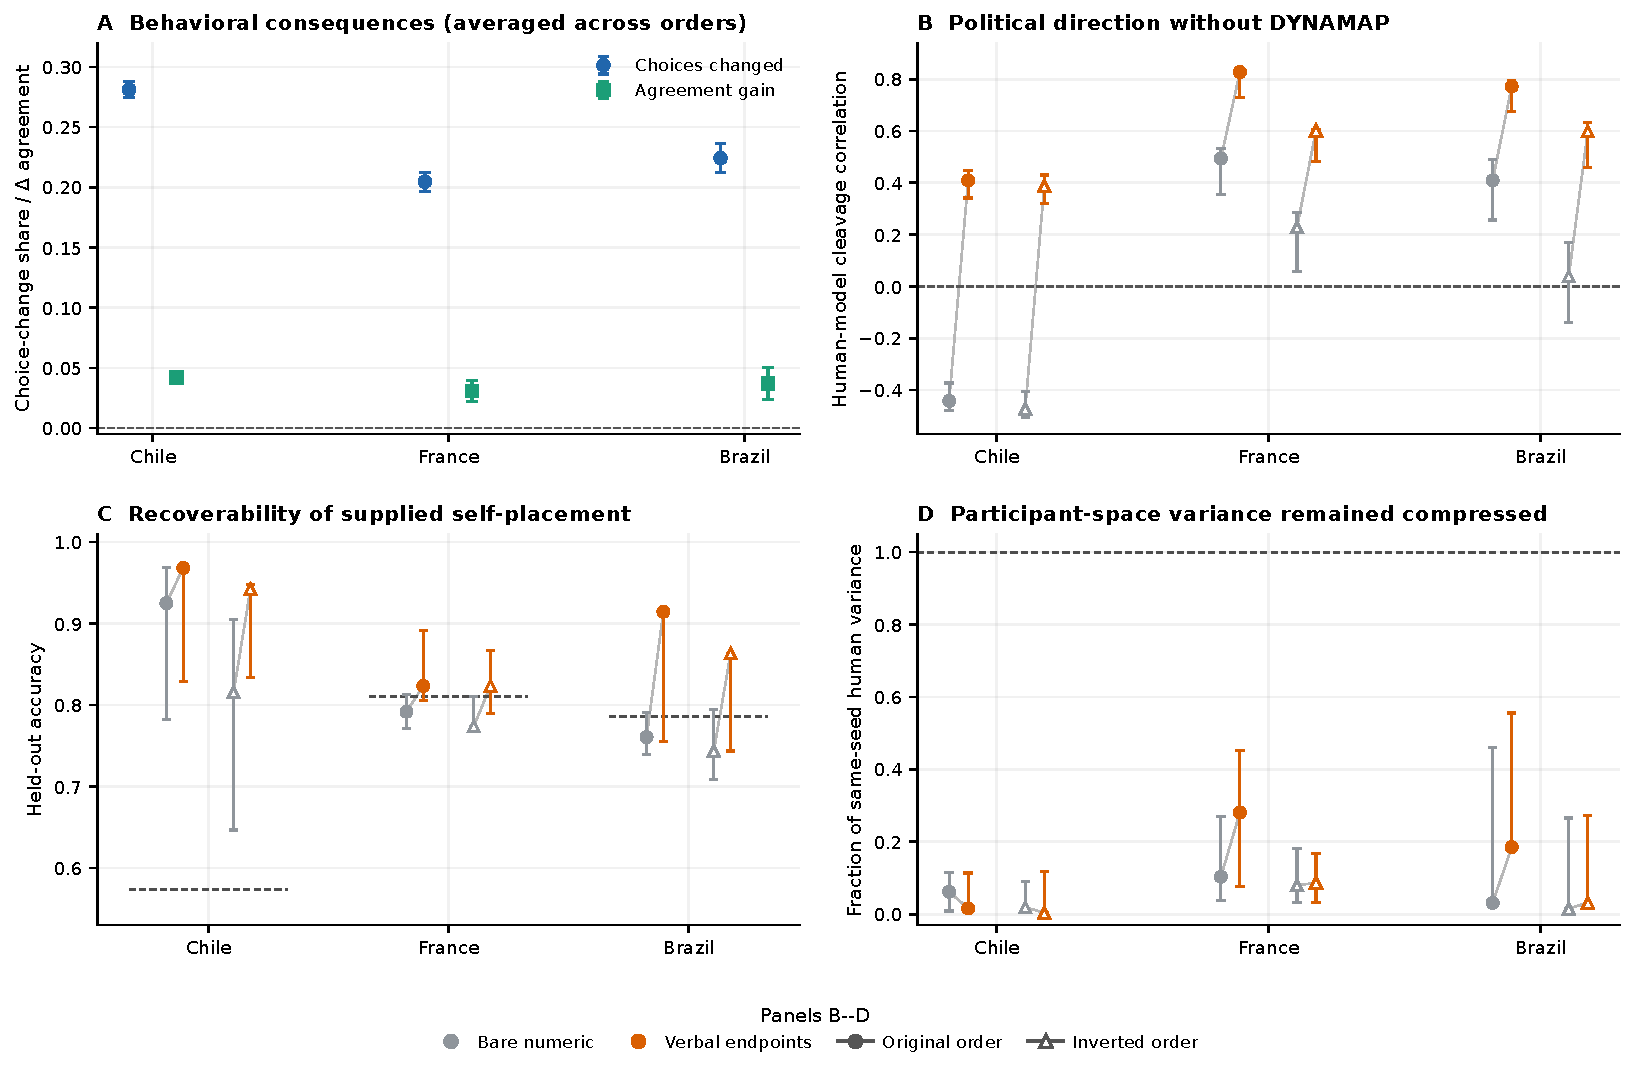
\includegraphics[width=0.98\textwidth]{figure6_endpoint_anchor_probe.pdf}
\caption{Verbal endpoint anchors changed political organization without restoring human population geometry. The outcome-informed probe uses Qwen3-32B at $T=0$ on the confirmed-adult C20 cohorts. Panel A reports order-averaged choice changes and matched-agreement gains with paired participant-bootstrap 95\% intervals; its dashed zero line denotes no agreement gain. Panel B reports human--model Bradley--Terry cleavage correlations for bare and anchored prompts in original (circles) and inverted (triangles) displays; intervals are paired participant-cluster bootstraps. Panels C--D show seed-101 points and 5th--95th percentiles across 30 DYNAMAP initialization seeds. Short dashed segments in panel C are country-specific held-out majority rules; the dashed line in panel D is the same-seed human variance. Anchors made the supplied axis more recoverable and moved cleavage toward the human direction, but did not restore human participant-space variance or remove order sensitivity.}
\label{fig:endpoint_anchor}
\figalttext[Four panels comparing bare numeric and verbally anchored self-placement prompts]{Verbal endpoints change roughly one fifth to more than one quarter of choices, modestly improve average human agreement, move political-cleavage correlations toward the human direction, and increase recoverability of supplied self-placement. Participant-space variance remains far below the human reference and differs between original and inverted proposal order.}
\end{figure*}

\section{Discussion}

Across the same matched decisions, criteria routinely collapsed into one accuracy score came apart. LLM conditions remained below several fitted human predictors while occupying much narrower participant-level spaces. Compression was the stable result: for every focal checkpoint in every setting, and across all 30 primary robustness seeds, synthetic participants spanned less of the latent space than the matched human participants. The endpoint probe preserved this result in all 372 bare and anchored model fits spanning seed 101 and 30 robustness initializations. Political organization was more contingent. Bare numeric prompts yielded an inverted Chilean cleavage and weaker French and Brazilian correspondence, but verbal endpoints moved all three toward the human direction while leaving the participant spaces compressed and position-sensitive. A single accuracy score or model leaderboard would conceal both the robust contraction and the fragility above it.

This separation extends evidence that plausible synthetic averages can coexist with under-dispersion and altered relationships \citep{Bisbee2024}, that demographic personas can be flattened or stereotyped \citep{Wang2025}, and that persona-conditioned behavioral spaces can contract across models and tasks \citep{Ball2025,Xiao2026,Bhattacharyya2026}. Our comparisons hold participants and proposals fixed within each setting, and every one of the 270 focal same-seed refits preserved lower synthetic participant variance than the paired human fit. The strongest claim is consequently specific: these LLM choices compress the breadth of participant-level DYNAMAP geometry across the evaluated checkpoints and settings.

That claim does not extend automatically to aggregate political structure. DYNAMAP participant variance measures how broadly people are distributed after proposal-anchor alignment; Bradley--Terry cleavage measures differences in marginal proposal utilities between political groups. Synthetic proposal utilities were often more dispersed than human utilities, while cleavage could be attenuated, amplified, or directionally misaligned. The endpoint intervention establishes that cleavage is also prompt-sensitive: a one-line clarification changed its direction and magnitude without eliminating geometric compression. Political differentiation can therefore be regular and pronounced without preserving either the same individual choices or a human-like population distribution.

The mechanism probe resolves one ambiguity but not the others. Omitting verbal endpoints contributed to the bare-prompt political mismatch: adding them moved cleavage toward the human direction in all six country-by-order comparisons. This is evidence about specification, not proof that scale interpretation alone generated every difference, because the checkpoint was selected after the original pattern was known and the two prompts were executed in separate deterministic runs. Instrument composition may also matter: the Chilean catalogue represented a 2019 domestic agenda, and delete-one-topic refits show that proposal topology is sensitive to which domains are retained. National political content may be represented unevenly in model training data, a possibility consistent with prior evidence but not testable from these responses alone \citep{Santurkar2023,Atari2023,Lu2025}. A fully crossed translation of one fixed instrument into Spanish, French, and Portuguese would vary language while holding participants and policy content constant; distinguishing training-data representation would additionally require independent corpus evidence or preregistered political-knowledge probes.

The interventions identify two further boundaries. Including self-placement increased its recoverability while slightly reducing matched human agreement in the fixed factorial; adding endpoints later made that supplied cue still more legible and modestly improved order-averaged agreement. Neither result is emergent inference or superior knowledge of the person \citep{Bernardelle2025}. Reversing A/B content and position changed 16.6--31.2\% of Chilean and 12.3--30.2\% of French and Brazilian choices in the factorial, and the anchored probe remained order-sensitive. Temperature-zero decoding therefore did not make substantive preferences position-invariant.

Cross-country differences still do not identify a training-data or country-level mechanism: language, policy instruments, institutions, election contexts, and sample composition vary together. The replication establishes that compression and sensitivity recur across settings; it does not establish why their magnitudes differ. The nonuniform endpoint effects provide a concrete example of why LLM evaluations established in one language or setting need not transfer unchanged to another \citep{Atari2023}. The human samples were voluntary online participants rather than national probability samples, and the personas included age, recorded sex, and self-placement rather than the full biographical and social context that differentiates people. Sparse personas can mechanically restrict model-based heterogeneity because deterministic responses are functions of the prompt-visible profile and displayed pair. Yet participants sharing a profile usually received different proposal sequences, so within-profile coordinate variation also contains item-composition variation; a balanced repeated-item design within identical profiles would be required to identify a persona-based variance ceiling.

These results do not invalidate LLM use in social research. Prediction, data augmentation, instrument stress testing, and evaluations of model representations answer different questions and may be useful in their intended settings \citep{GudinoRosero2024}. The evidence instead limits claims of participant substitution. DYNAMAP reconstruction concerns observed participants and proposals, not cold-start prediction; participant-bootstrap intervals condition on observed policy instruments; and most geometry estimates condition on fitted networks. Model implementations also differed across families. Broader-C10, policy-domain, topic-deletion, and sequential-context analyses in the SI Appendix preserve the central diagnosis while delimiting its generality.

The appropriate unit of validation is therefore the checkpoint--prompt--setting combination: each component moved distinct fidelity criteria in these data, consistent with evidence that survey wording and response-generation method can materially alter LLM survey behavior \citep{Tjuatja2024,Ahnert2026}. We propose the following evaluation standard for simulated publics: compare internal reconstruction with a naive baseline; benchmark matched choices against out-of-sample human predictors; specify scale endpoints explicitly; ablate focal persona information; counterbalance proposal position; and separately measure participant heterogeneity, proposal topology, and political cleavage. Internally regular or politically classifiable responses should not be treated as human substitutes without independent evidence of matched-choice, positional, population-level, and relational fidelity in the specific setting of use.

\section{Materials and methods}

\subsection{Human data and fixed matched design}

The Chilean source table contained 3,007,714 pairwise decisions from 48,119 participant records over 90 policy proposals. We retained participants with one profile row, valid political self-placement and age, and at least 20 eligible decisions after excluding records flagged as nonpolitical. This yielded 31,763 eligible participants and 2,311,464 decisions. With seed 20260821, we drew a fixed frame of 2,000 anonymous participant identifiers (UUIDs) without replacement and retained each participant's first 20 eligible decisions chronologically. The confirmed-adult cohort then restricted that frame to the 1,991 participants with an exact reported age of at least 18, yielding 39,820 decisions. It included 674 participants recorded as female, 1,310 as male, and seven in another category; mean age was 36.4 years (SD, 10.8). The Chilean instrument defined positions 1--4 as left, 5 as center, and 6--10 as right. Binary left--right analyses used 653 left- and 503 right-identifying adults; the 835 midpoint participants were excluded only from those binary contrasts and retained in every other analysis. UUIDs linked records but never entered prompts. Except for the cohort-construction counts in this paragraph, every reported sample size and estimate in the main text and SI Appendix refers to the confirmed-adult cohorts.

\subsection{Model grid, personas, and inference}

The grid crossed three instruction-tuned model families and three checkpoint sizes: Qwen3 (8B, 14B, and 32B), Gemma 4 (E4B, 12B, and 31B), and Ministral 3 (3B, 8B, and 14B). Exact model identifiers, repository revisions, inference engines, and numerical formats are reported in SI Appendix, Table~S1. Open-weight checkpoints were chosen because immutable revisions and local inference settings permit exact replay; this design does not represent hosted proprietary systems. Because families differed in training, architecture, serving software, and precision, cross-family comparisons are descriptive rather than causal effects of parameter count.

The Spanish system message situated the decision in Chile in 2019, prohibited invented attributes and later information, required one choice, and prohibited explanation. The user message supplied age, recorded sex, political self-placement, and the two proposal texts. The response contract admitted only A or B. UUIDs, human choices, coordinates, timestamps, proposal popularity, and prior decisions were excluded. Reasoning was disabled. Each checkpoint was evaluated at $T\in\{0,0.2,0.7\}$ with top-$p=1$ and fixed generation seeds documented in the SI Appendix. Because each condition contains one draw per decision cell, temperature is evaluated as a decoding intervention and not as a proxy for human heterogeneity. Verbatim templates in Spanish, French, and Portuguese appear in the SI Appendix.

\subsection{Factorial interventions and response decoding}

From the completed grid, we selected three temperature-zero checkpoints representing different diagnostic maxima: Gemma 4-12B for matched human agreement, Qwen3-32B for self-placement recoverability, and Ministral 3-14B for DYNAMAP lift. This checkpoint selection was outcome-informed. Before generating the intervention responses, we fixed a $2\times2$ design crossing political self-placement present versus ablated with original versus content-and-position-inverted A/B display. The balanced design comprised 12 cells; nine were newly generated and three exact original-order, self-placement-present cells were reused after verifying identity and completeness. The stored responses were projected onto the same confirmed-adult UUID manifest, so every analyzed cell contained 1,991 participants and 39,820 decisions.

In inverted cells, displayed A contained the original B proposal and displayed B contained the original A proposal. All responses were decoded to original proposal identity before substantive comparisons. The self-placement effect is present minus ablated within checkpoint and order; the position effect is inverted minus original within checkpoint and prompt condition. Behavioral intervals used 2,000 paired bootstrap replicates that resampled adults with their complete 20-decision histories. Classification contrasts were recalculated on the adult coordinate fits with the fixed split and folds described below.

All 12 cells used the same two-dimensional DYNAMAP architecture, primary initialization seed 101, 20 epochs, and decisions 1--18/19--20 training--validation split as the grid. Political-self-placement validation used the same random forest with 2,000 estimators and seed 42. Primary-fit geometry intervals are post-fit: they resample participants or proposal pairs while holding one fitted coordinate system fixed. Optimization sensitivity was assessed separately with repeated DYNAMAP refits.

\subsection{France--Brazil cross-country replication}

The cross-country replication used policy choices collected through an online participation platform during the 2022 French and Brazilian presidential elections \citep{Navarrete2023Data,Navarrete2024}. Cleaning required nonmissing participant, pair, selected-proposal, and timestamp fields; two distinct catalogue-backed proposals; a selected item present in the pair; \texttt{suspicious=0}; the latest valid observation per participant and unordered proposal pair; and the latest usable profile with documented age, sex, and political self-placement. Age was released in bands. To ensure adult-only scope, we excluded the entire 10--19 band because ages 18--19 could not be separated from younger respondents. The primary C20 cohorts therefore comprised 843 confirmed adults and 16,860 rows in France, and 434 confirmed adults and 8,680 rows in Brazil. Decisions 1--18 trained DYNAMAP and 19--20 were held out. A broader confirmed-adult C10 sensitivity included 847 French and 515 Brazilian participants and used decisions 1--8/9--10. Because C10 changes both cohort membership and training volume, it is not a causal history-length intervention.

The same three checkpoints and temperature-zero stateless factorial were rendered in French and Brazilian Portuguese using native proposal text and the 2022 context. French and Brazilian five-point self-placement was grouped as 1--2 left/center-left, 3 center, and 4--5 center-right/right; scales were interpreted only within country. Stored responses were projected onto the confirmed-adult C20 and C10 UUID manifests before analysis; no model inference was repeated for the age restriction. Released human records place the selected proposal first, yielding an outcome-informed released-file order rather than verified historical display position. We therefore decoded every response to proposal identity and used the equal-weight average over all four self-placement-by-order cells as the primary agreement estimate. Cross-order consistency compared proposal identity in paired original and inverted rows with 2,000 participant-bootstrap resamples.

\subsection{Verbal endpoint-anchor mechanism probe}

After inspecting the bare-numeric results, we ran an outcome-informed diagnostic with Qwen3-32B at $T=0$ in Chile, France, and Brazil. It reused the confirmed-adult C20 cohorts and the exact original and inverted decision keys. Model revision, runtime, numerical format, system message, persona fields, proposal text, response contract, and decoding parameters were held fixed. The only prompt change appended verbal endpoints to the self-placement line: ``1 = extrema izquierda; 10 = extrema derecha'' in Chile, ``1 = extr\^{e}me gauche; 5 = extr\^{e}me droite'' in France, and ``1 = extrema esquerda; 5 = extrema direita'' in Brazil. Six new cells were paired with their existing bare-numeric controls and decoded to original proposal identity.

Behavioral and Bradley--Terry contrasts used 2,000 paired UUID-cluster bootstrap replicates. DYNAMAP was refitted independently for bare and anchored responses using the same C20 split and estimator specification. Seed 101 provides the manuscript-compatible point estimates; 30 additional paired initializations refitted every model condition against the same-seed national human reference. These seed distributions quantify optimization sensitivity conditional on fixed model responses. Because the checkpoint and intervention were selected after the earlier pattern was observed, this probe tests a candidate mechanism and does not estimate a general effect of verbal anchoring across checkpoints.

\subsection{Behavioral, classification, and uncertainty estimands}

Matched human agreement equals one when a model selected the substantive proposal chosen by the corresponding human participant. In inverted cells it was computed only after decoding the displayed response to original proposal identity. Original-A rate measures selection of that original proposal identity, whereas displayed-A rate diagnoses positional response concentration. Participant-level response entropy and persistence were calculated on explicitly identified decoded or displayed outcomes. Confidence intervals used 2,000 bootstrap replicates resampling participants with complete histories; no analysis treated decision rows as independent.

For a common Chilean behavioral benchmark, decisions 1--18 trained reference predictors and decisions 19--20 (3,982 adult choices) evaluated balanced random choice, the training-set marginal A/B rule, Bradley--Terry proposal popularity \citep{Bradley1952}, a sociodemographic-plus-proposal-identity classifier, and human DYNAMAP on the same held-out cells. Balanced random accuracy is the analytic value 0.500 and therefore has no sampling interval. Comparable LLM outputs were evaluated on those cells after response decoding where required.

Self-placement recoverability was evaluated after excluding only each country's midpoint category. Random forests with 2,000 trees, entropy splits, and seed 42 predicted binary left versus right self-placement from archived sociodemographic fields, then from those fields plus the two DYNAMAP coordinates. We report a fixed, unstratified 70/30 holdout together with stratified 10-fold cross-validation. The fixed holdout is preserved to avoid post-result redefinition; balanced accuracy, macro-F1, ROC AUC, and stratified CV-10 provide class-imbalance and partition sensitivities. Coordinate gain is the difference between augmented and sociodemographic-only held-out accuracy; it is distinct from absolute classification performance. Because self-placement was supplied in one factorial arm, this analysis measures recoverability of a supplied or ablated cue rather than emergent political inference.

Participant-bootstrap intervals condition on the observed proposal set. As a sensitivity analysis, a crossed Poisson-pigeonhole bootstrap applied product weights to participants, proposal A, and proposal B. This approximates uncertainty under proposal interchangeability but does not turn the observed policies into a probability sample of a defined policy universe.

\subsection{DYNAMAP reconstruction}


Human and synthetic spaces were fitted independently with the same two-dimensional DYNAMAP architecture. DYNAMAP jointly learns participant and proposal coordinates from repeated pairwise choices, with all coordinates constrained to $(0,1)$ by a componentwise sigmoid. Choice prediction uses the elementwise squared participant--proposal displacements as inputs to a flexible shared-parameter neural head, rather than imposing a monotonic Euclidean-distance choice rule. The complete choice function and its parameter sharing are specified in the SI Appendix (\textit{DYNAMAP architecture and validation}). Models minimized binary cross-entropy with Adamax (learning rate 0.01), batch size 64, no epoch shuffling, primary initialization seed 101, and 20 epochs. In C20, decisions 1--18 trained the model and decisions 19--20 formed within-participant validation sets of 3,982 Chilean, 1,686 French, and 868 Brazilian rows. C10 used decisions 1--8/9--10. We report accuracy, the validation-set majority-label accuracy, and their difference (lift). These are deterministic validation-set point diagnostics conditional on a fitted model; initialization sensitivity is reported separately rather than as participant-sampling confidence intervals. They measure reconstruction for observed participants and items, not matched human fidelity or prediction for new participants.

\subsection{Alignment, geometry, and independent validation}

Because independently learned coordinates are arbitrary up to orientation and scale, each synthetic proposal matrix---90 items in Chile, 120 in France, and 67 in Brazil---was mapped to its own country's human proposal matrix with a least-squares similarity Procrustes transformation \citep{Schonemann1966}. The fitted rotation or reflection, scale, and translation were then applied unchanged to participant coordinates; political self-placement did not enter alignment, and spaces were never aligned across countries. We measured left--right participant-centroid distance, total participant covariance trace, and the Pearson correlation between all matched pairwise proposal distances. The first two were normalized to the corresponding human value.

Optimization sensitivity varied only the DYNAMAP initialization across 30 fixed seeds for the confirmed-adult C20 human samples and the three focal temperature-zero, self-placement-present, original-order model conditions in each country. Human and synthetic spaces were refitted at the same seed before alignment, yielding 270 focal synthetic--human comparisons. These distributions quantify sensitivity to DYNAMAP optimization, not uncertainty in model generation or participant sampling. Broader-C10, policy-domain, topic-deletion, and sequential-context analyses are reported in the SI Appendix; the sequential analysis is compared only with its matched local stateless implementation.

To ensure that proposal-level political conclusions did not depend on the DYNAMAP embedding, we fitted L2-regularized Bradley--Terry logistic models without an intercept to aggregate proposal choices. We report proposal-score and rank correlations, pairwise ordering agreement, and synthetic-to-human root-mean-square score dispersion. Political cleavage was estimated by fitting the same model separately to left- and right-identifying participants and defining each proposal's cleavage as centered right-group minus left-group utility. Human and synthetic cleavage vectors were compared by Pearson and Spearman correlation, sign agreement, slope through the origin, and relative root-mean-square magnitude. Two thousand paired participant-cluster bootstrap replicates refitted the human and synthetic models with identical multiplicities. DYNAMAP participant variance, aggregate proposal dispersion, and political cleavage are distinct estimands and need not move together.

% \subsection{Reproducibility}

% All analyses use versioned source extracts with recorded checksums and fixed condition definitions. Exact checkpoint revisions, inference engines, numerical formats, decoding parameters, random seeds, cohort rules, and estimator specifications are documented in the SI Appendix. Human and synthetic responses are joined through anonymous decision keys, and content-inverted responses are decoded to proposal identity before analysis. Machine-readable source tables accompany the figures and tables, and the reproduction workflow separates inference, statistical estimation, and manuscript rendering. Direct identifiers and private participant-level joins are excluded from shared materials. OpenAI Codex was used during August--September 2026 for code generation, debugging, and reproducibility checks, and OpenAI ChatGPT (GPT-5.6 Sol) for language editing and consistency checking; all AI-assisted outputs were reviewed and verified by the authors.

\section*{Use of generative AI}

OpenAI Codex and ChatGPT (GPT-5.6 Sol; OpenAI) assisted with code review, consistency checks, and editorial revision during August–September 2026. The authors specified the analyses, reviewed the generated code and text, verified the numerical outputs, and take responsibility for all results and content.

\section*{Ethics and informed consent}

This study is based exclusively on secondary analysis of previously collected anonymous data and involved no new participant recruitment, interaction, or data collection. Participation in the original online platforms was voluntary and uncompensated. The datasets contain session-generated identifiers used to link responses within the platforms, but no names, national identification numbers, email addresses, or other direct personal identifiers were collected.

The French and Brazilian data were collected through the MonProgramme2022 and Brazucracia platforms under ethics-approved protocols, with participants accepting the platforms' consent form, as documented in the original study \citep{Navarrete2024}. The Chilean data were collected through the Chilecracia online civic-participation platform. The secondary analysis reported here was reviewed by the Institutional Ethics Committee of Universidad del Desarrollo, which determined that it was exempt from full ethical review on June 24, 2025.

\section*{Acknowledgments}

The authors have no additional acknowledgments to report.

\section*{Funding}

The authors acknowledge financial support from the Instituto de Data Science, Universidad del Desarrollo. C.C. acknowledges financial support from Agencia Nacional de Investigación y Desarrollo (ANID), FONDECYT Regular grant no. 1262601.


\section*{Author contributions}

A.F.-J.: Conceptualization, Methodology, Investigation, Software, Formal analysis, Data curation, Validation, Visualization, Project administration, Writing---original draft, Writing---review and editing. C.C.: Conceptualization, Methodology, Supervision, Resources, Writing---review and editing.

\section*{Conflicts of interest}

The authors declare a competing interest. A.F.-J. and C.C. are named inventors on a pending U.S. patent application related to the DYNAMAP framework described in this article and assigned to Universidad del Desarrollo.

\section*{Data availability}

The France and Brazil datasets analyzed in this study are publicly available through \href{https://doi.org/10.7910/DVN/8E0EA4}{Harvard Dataverse (DOI: 10.7910/DVN/8E0EA4)} \citep{Navarrete2023Data}. The Chilean dataset was originally collected through a publicly accessible online platform that is no longer active; an archived description of the platform and its data is available through the \href{https://web.archive.org/web/20191229112008/https://chilecracia.org/datos}{Internet Archive}. The \href{https://github.com/adolfofuentesjofre/DYNAMAP}{public DYNAMAP repository} provides a reduced Chilean replication dataset and selected fitted outputs. Cleaned analytical data, prompt materials, validated model responses, environment specifications, and derived outputs for the present study are available from the corresponding author during review, subject to ethical and data-protection considerations, and will be deposited in a public repository upon acceptance. Direct identifiers and private participant-level joins will not be released.

\section*{Code availability}

The DYNAMAP implementation and reduced replication materials are available at \href{https://github.com/adolfofuentesjofre/LLMs_Compress_human_preference_geometry}{github.com/adolfofuentesjofre/LLMs}. Analysis code specific to the present study is available from the corresponding author during review and will accompany the public repository deposit upon acceptance.

\bibliographystyle{oup-plain}
\bibliography{references}

\end{document}
